\documentclass[12pt,aspectratio=169]{beamer}
\usetheme{metropolis}
\setbeamersize{text margin left=.5cm,text margin right=.5cm}
\usepackage[lf]{carlito}
\usepackage{tikz}
\usepackage{mathpazo}
\usepackage{xcolor,colortbl}
\usepackage{siunitx}

\setlength{\parskip}{0pt}
\renewcommand{\baselinestretch}{1}

\sisetup{
  per-mode=symbol
}
\tikzset{>=latex}

\title{Topic 12: Capacitors}
\subtitle{Advanced Placement Physics 2}
\author[TML]{Dr.\ Timothy Leung}
\institute{Olympiads School}
\date{Last Updated: \today}

\newcommand{\pic}[2]{\includegraphics[width=#1\textwidth]{#2}}
\newcommand{\mb}[1]{\mathbf{#1}}
\newcommand{\eq}[2]{\vspace{#1}{\Large\begin{displaymath}#2\end{displaymath}}}


\begin{document}

\begin{frame}
  \maketitle
\end{frame}


%\begin{frame}{Files for You to Download}
%  Please download these files from the school website if you have not already
%  done so:
%  \begin{enumerate}
%  \item\texttt{PhysAPC-12-Capacitors.pdf}---This presentation. If you want to
%    print on paper, I recommend printing 4 pages per side.
%  %\item\texttt{09-10-Homework.pdf}---Homework assignment for Topics 9
%  %  (electrostatics) and 10 (Gauss' law).
%  \end{enumerate}
%
%  \vspace{.2in}Please download/print the PDF file \emph{before} each class.
%  There is no point copying notes that are already printed out for you.
%  Instead, take notes on things I say that aren't necessarily on the slides.
%\end{frame}



\section{Capacitors}


%\begin{frame}{Electric Field and Electric Potential Difference}
%  Recall that the relationship between electrostatic force ($\mb{F}_q$) and
%  electric potential energy ($U_q$) can be expressed using definition of
%  mechanical work and the fundamental theorem of calculus:
%
%  \eq{-.25in}{
%    \Delta U_q=-\int\mb{F}_q\cdot d\mb{r}\quad\quad
%    \mb{F}_q=-\nabla U_q=-\frac{\partial U_q}{\partial r}\hat{\mb{r}}
%  }
%
%  \vspace{-.08in}Dividing both sides of the equations by $q$, we get the
%  relationship between electric field ($\mb{E}$), electric potential ($V$) and
%  electric potential difference ($\Delta V$):
%  
%  \eq{-.2in}{
%    \Delta V=-\int\mb{E}\cdot d\mb{r}\quad\quad
%    \boxed{\mb{E}=-\nabla V=-\frac{\partial V}{\partial r}\hat{\mb{r}}}
%  }
%
%  This relationship holds regardless of the charge configuration.
%\end{frame}




\begin{frame}{Electric Field and Electric Potential Difference}
  \begin{center}
    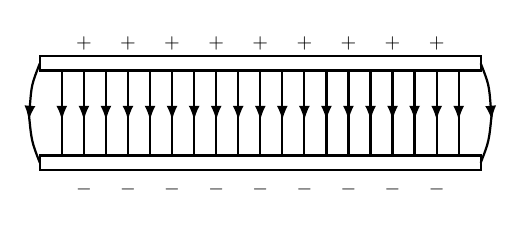
\begin{tikzpicture}[xscale=.7,yscale=.9]
      \draw[thick](0,0) rectangle (8,.2);
      \draw[thick](0,1.4) rectangle (8,1.6);
      \foreach\x in {.4,.8,1.2,...,7.6}{
        \draw[->,thick](\x,1.4)--(\x,.7);
        \draw[thick](\x,1.4)--(\x,.2);
      }
      \foreach\x in {.8,1.6,2.4,...,7.2}{
        \node at (\x,1.78) {\scriptsize $+$};
        \node at (\x,-.28) {\scriptsize $-$};
      }
      
      \draw[->,thick](0,1.5)..controls(-.15,1.2)..(-.2,.7);
      \draw[thick](-.2,.8)..controls(-.15,.4)..(0,.1);

      \draw[->,thick](8,1.5)..controls(8.15,1.2)..(8.2,.7);
      \draw[thick](8.2,.8)..controls(8.15,.4)..(8,.1);
    \end{tikzpicture}
  \end{center}
  \vspace{-.1in}Recall that for two charged parallel plates, the electric field
  is uniform, and the relationship between electric field and potential
  difference simplifies to:

  \eq{-.2in}{
    \boxed{E=\frac{\Delta V}{d}}
    \quad\text{or}\quad
    \boxed{\Delta V=Ed}
  }
  \begin{center}
    \begin{tabular}{l|c|c}
      \rowcolor{pink}
      \textbf{Quantity} & \textbf{Symbol} & \textbf{SI Unit} \\ \hline
      Electric field intensity & $E$ & \si{\newton\per\coulomb}\\
      Electric potential difference between plates & $\Delta V$ &
      \si{\volt} \\
      Distance between plates       & $d$ & \si{\metre}
    \end{tabular}
  \end{center}
\end{frame}



\begin{frame}{Capacitors}
  \textbf{Capacitors} is a device that stores energy in an electric field. The
  simplest form of a capacitor is a set of closely spaced parallel plates:
  \begin{center}
    \pic{.5}{cap19}
  \end{center}
  When the plates are connected to a battery, the battery transfer charges to
  the plates until the voltage $V$ equals the battery terminals. After that,
  one plate has charge $+Q$; the other has $-Q$.
\end{frame}



\begin{frame}{Parallel-Plate Capacitors}
  As we have seen already, the (uniform) electric field between two parallel
  plates is proportional to the charge density $\sigma$, which is the charge
  $Q$ divided by the area of the plates $A$:

  \eq{-.2in}{
    E=\frac{\textcolor{red}{\sigma}}{\epsilon_0}=
    \frac{\textcolor{red}{Q}}{\textcolor{red}{A}\epsilon_0}
  }
  
  Substituting this into the relationship between the plate voltage $V$ and
  electric field, we find a relationship between the charges across the plates
  and the voltage:

  \eq{-.2in}{
    V=\textcolor{blue}{E}d=
    \frac{\textcolor{blue}{Q}d}{\textcolor{blue}{A\epsilon_0}}
    \quad\longrightarrow\quad
    \boxed{Q=\left[\frac{A\epsilon_0}{d}\right]V}
  }
\end{frame}



\begin{frame}{Parallel-Plate Capacitors}
  Since area $A$, distance of separation $d$ and the vacuum permittivity
  $\epsilon_0$ are all constants, the relationship between charge $Q$ and
  voltage $V$ is \emph{linear}. And the constant is called the
  \textbf{capacitance} $C$, defined as:

  \eq{-.15in}{
    \boxed{C=\frac{Q}{V}}
  }

  For parallel plates:

  \eq{-.2in}{
    C=\frac{A\epsilon_0}{d}
  }

  The unit for capacitance is a \textbf{farad} (named after Michael Faraday),
  where $\SI{1}{\farad}=\SI{1}{\coulomb\per\volt}$.
\end{frame}


%\begin{frame}{Parallel-Plate Capacitors}
%  Capacitance $C$ is defined as the ratio between charge $Q$ ($+$ on one
%  plate; $-$ on the other) and potential difference (voltage) $V$:
%  
%  \eq{-.05in}{
%    \boxed{C=\frac{Q}{V}}
%  }
%  
%  \begin{center}
%    \begin{tabular}{l|c|l}
%      \rowcolor{pink}
%      \textbf{Quantity} & \textbf{Symbol} & \textbf{SI Unit} \\ \hline
%      Capacitance   & $C$   & \si{\farad} (farads)\\
%      Charge        & $Q$   & \si{\coulomb} (coulombs)\\
%      Voltage across the plates & $V$ & \si{\volt} (volts)
%    \end{tabular}
%  \end{center}
%\end{frame}



\begin{frame}{Practical Capacitors}
  \begin{columns}
    \column{.3\textwidth}
    \pic{1.15}{Figure_20_05_05a}
    \column{.7\textwidth}
    \begin{itemize}
    \item Parallel-plate capacitors are very common in electric circuits,
      but the vacuum between the plates is not very effective
    \item Instead, a non-conducting \textbf{dielectric} material is inserted
      between the plates
    \item When the plates are charged, the electric field of the plates
      polarizes the dielectric.
    \item The polarization  produces an electric field that opposes the field
      from the plates, therefore reduces the effective voltage, and increasing
      the capacitance
    \end{itemize}
  \end{columns}
\end{frame}



\begin{frame}{Dielectric Constant}
  If electric field without dielectric is $E_0$, then $E$ in the dielectric is
  reduced by $\kappa$, the \textbf{dielectric constant}:

  \eq{-.25in}{
    \boxed{\kappa=\frac{E_0}{E}}
  }

  The capacitance of the plates with the dielectric is now amplified by the
  same factor $\kappa$:

  \eq{-.3in}{
    \boxed{C=\kappa C_0}
  }

  We can also view the dielectric as something that increases the
  \emph{effective permittivity}:
  
  \eq{-.3in}{
    \boxed{\epsilon=\kappa\epsilon_0}
  }
\end{frame}



\begin{frame}{Dielectric Constant}
  The dielectric constants of commonly used materials are:
  \begin{center}
    \begin{tabular}{l|l}
      \rowcolor{pink}
      \textbf{Material} & $\kappa$ \\ \hline
      Air         & \num{1.00059} \\
      Bakelite    & \num{4.9} \\
      Pyrex glass & \num{5.6} \\
      Neoprene    & \num{6.9} \\
      Plexiglas   & \num{3.4} \\
      Polystyrene & \num{2.55} \\
      Water (\SI{20}{\celsius}) & \num{80} 
    \end{tabular}
  \end{center}
\end{frame}


\begin{frame}{Storage of Electrical Energy}
  \begin{center}
    \pic{.45}{slide14}
  \end{center}
  \begin{itemize}
  \item When charging up a capacitor, imagine positive charges moving from the
    negatively charged plate to the positively charged plate
  \item Initially neither plates are charged, so moving the first charge takes
    very little work; as the electric field builds, more and more work needs
    to be done
  \end{itemize}
\end{frame}



\begin{frame}{Storage of Electrical Energy}
  \begin{center}
    \pic{.35}{slide14}
  \end{center}
  \begin{itemize}
  \item In the beginning---when the plates aren't charged---moving a very
    small\footnote{\emph{infinitesimal}, in math speak} charge $dq$ across
    the plates, the infinitesimal work done $dU$ is very small
  \item As the electric field begins to form between plates, more and more work
    is required to move the charges.
  \end{itemize}
\end{frame}



\begin{frame}{Storage of Electrical Energy}
%  To fully charge the plates, the total work $U_c$ is the integral:
%
%  \eq{-.2in}{
%    U_c=\int dU=\int_0^Q\frac{q}{C}dq=\frac{1}{2}\frac{Q^2}{C}
%  }
%
  With some calculus, we can find the work done is stored as a potential energy
  inside the capacitor. There are different ways to express $U_c$ using
  definition of capacitance:

  \eq{-.15in}{
    \boxed{U_c=\frac12\frac{Q^2}{C}=\frac12QV=\frac12CV^2}
  }
\end{frame}




\begin{frame}{Notes About Storage of Electric Energy}
  \begin{itemize}
  \item The work done (i.e.\ the energy stored in the capacitor) is inversely
    proportional to the capacitance:

    \eq{-.2in}{
      dU=Vdq=\frac{q}{C}dq
    }
  \item The presence of a dielectric \emph{increases} the capacitance; therefore
    the work (and potential energy stored) to move the charge $dq$
    \emph{decreases} with the dielectric constant $\kappa$
  \item After the capacitor is charged, removing the dielectric material from
    the capacitor plates will require additional work.
  \end{itemize}
\end{frame}

\end{document}
